\documentclass{article}

\usepackage{tikz}
\usetikzlibrary{decorations.pathmorphing}
\usetikzlibrary{patterns}
\usetikzlibrary{arrows.meta}

\begin{document}
    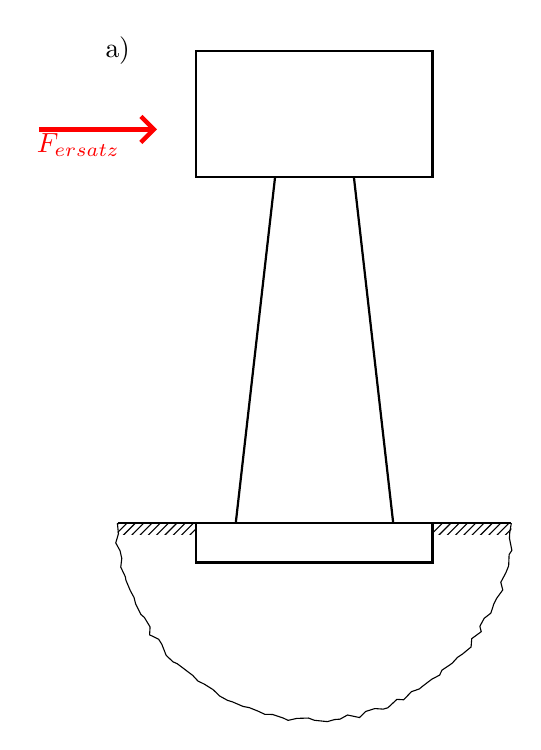
\begin{tikzpicture}[pencildraw/.style={
        black,
        decorate,
        decoration={random steps,segment length=3pt,amplitude=1pt}
        }]

        %Building
        \draw[black, thick] (0,0.4) rectangle (3,2);
        \draw[black, thick] (1,0.4) -- (0.5, -4);
        \draw[black, thick] (2,0.4) -- (2.5, -4);
        \draw[black, thick] (0, -4.5) rectangle (3, -4);

        %Text
        \draw[-{Straight Barb}, red, ultra thick] (-2,1) -- (-0.5, 1);
        \node[font = \bfseries, text = red, align = left] at (-1.5,0.8) {$F_{ersatz}$};
        \node at (-1,2) {a)};

        %Ground
        \draw[black, thick] (-1, -4) -- (4, -4);
        \draw[pencildraw] (4, -4) arc (0:-180:2.5);
        \draw[pattern = north east lines, draw = none] (-1, -4.15) rectangle (0, -4);
        \draw[pattern = north east lines, draw = none] (3, -4.15) rectangle (4, -4);
        
    \end{tikzpicture}
\end{document}